%----------------------------------------------------------------
%
%  File    :  thesis.tex
%
%----------------------------------------------------------------

% --- Setup for the document ------------------------------------

%Class for a book like style:
\documentclass[11pt,a4paper,oneside]{scrbook}
%For a more paper like style use this class instead:
%\documentclass[11pt,a4paper,oneside]{thesis}

%input encoding for windows in utf-8 needed for Ä,Ö,Ü etc..:
\usepackage[utf8]{inputenc}
%input encoding for linux:
%\usepackage[latin1]{inputenc}
%input encoding for mac:
%\usepackage[applemac]{inputenc}

\usepackage[english]{babel}
% for german use this line instead:
%\usepackage[ngerman]{babel}

%needed for font encoding
\usepackage[T1]{fontenc}

% want Arial? uncomment next two lines...
%\usepackage{uarial}
%\renewcommand{\familydefault}{\sfdefault}

%some formatting packages
\usepackage[bf,sf]{subfigure}
\renewcommand{\subfigtopskip}{0mm}
\renewcommand{\subfigcapmargin}{0mm}

%For better font resolution in pdf files
\usepackage{lmodern}

\usepackage{url}

\usepackage{glossaries}
\newglossaryentry{facade}
{
    name=facade,
    description={The Facade pattern is a software design pattern that provides a simplified interface to a larger body of code, making it easier to use and understand. It is a structural pattern that involves creating a single class, known as the facade, which acts as a front-facing interface for a complex system of classes and components.}
}
\newglossaryentry{FaaS}
{
    name=FaaS,
    description={FaaS stands for Function-as-a-Service, which is a cloud computing model where developers can create and deploy small, single-purpose functions that are executed on demand, in response to events or triggers.}
}
\newglossaryentry{serverless}
{
    name=serverless,
    description={Serverless computing is a cloud computing model in which the cloud provider manages the infrastructure and automatically allocates computing resources as needed to execute and scale applications. In a serverless architecture, developers write and deploy code as small, independent functions that are triggered by specific events or requests, such as an HTTP request. The cloud provider then executes these functions on its own infrastructure, dynamically allocating computing resources and scaling automatically to meet demand. Because the cloud provider manages the infrastructure and abstracts away the underlying hardware and software, developers do not have to worry about managing servers, scaling infrastructure, or paying for idle resources, which can lead to reduced operational costs and increased agility.}
}
\newglossaryentry{WebAssembly}
{
    name=Wasm,
    description={WebAssembly (abbreviated Wasm) is a safe, portable, low-level code format designed for efficient execution and compact representation. Its main goal is to enable high performance applications on the Web, but it does not make any Web-specific assumptions or provide Web-specific features, so it can be employed in other environments as well.}
}
\newglossaryentry{V8}
{
    name=V8,
    description={V8 is a high-performance JavaScript engine developed by Google for use in their Chrome web browser and other applications. It is also used by Node.js to execute JavaScript code outside of a web browser. V8 is written in C++ and compiles JavaScript code to native machine code, providing significant performance benefits over interpreted JavaScript engines.}
}
\newglossaryentry{isolate}
{
    name=isolate,
    description={The isolates runtime runs on the V8 engine, which is the same engine that powers Chromium and Node.js. The Workers runtime also supports many of the standard APIs that most modern browsers have.}
}
\newglossaryentry{LXC-Container}
{
    name=LXC-Container,
    description={LXC (Linux Containers) is a lightweight virtualization technology that allows multiple isolated Linux systems, known as containers, to run on a single Linux host. LXC-Containers provide a way to run applications in an isolated environment with their own file system, network interface, and resource allocation. Each LXC-Container shares the host operating system kernel but runs its own isolated user space.}
}
\newglossaryentry{edge computing}
{
    name=edge computing,
    description={Edge computing is the concept of bringing computation power closer to the end consumer. Due to the lower proximity between the server and the end device, this solution reduces network latency. Typical use cases are in the Internet of Things, mobile or gaming sectors where latency plays a huge role.}
}
\newglossaryentry{cloud computing}
{
    name=cloud computing,
    description={According to the National Institute of Standards and Technology (NIST) definition of cloud computing is a model for enabling ubiquitous, convenient, on-demand network access to a shared pool of configurable computing resources (e.g., networks, servers, storage, applications, and services) that can be rapidly provisioned and released with minimal management effort or service provider interaction. This cloud model is composed of five essential characteristics, three service models, and four deployment models \cite{mell_2011_the}.}
}
\newglossaryentry{wasi}
{
    name=WASI,
    description={The WebAssembly System Interface is not a monolithic standard system interface, but is instead a modular collection of standardized APIs. None of the APIs are required to be implemented to have a compliant runtime. Instead, host environments can choose which APIs make sense for their use cases \cite{webassembly_2023_webassemblywasi}.}
}
\newglossaryentry{LLVM}
{
    name=LLVM,
    description={A toolkit used to build and optimize compilers. The LLVM Project consists of a set of modular and reusable compiler and toolchain technologies, which form a collection that can be utilized across various compilers and toolchains.}
}
\newglossaryentry{POSIX}
{
    name=POSIX,
    description={Portable Operating System Interface is a set of standards defined by the IEEE for maintaining compatibility between operating systems.}
}
\newglossaryentry{libc}
{
    name=libc,
    description={Short for C Standard Library, it is a library of standard functions that are a part of the C programming language, which define the functions used for file operations, input and output operations, string manipulation, and memory allocation etc.}
}
\newglossaryentry{JS glue code}
{
    name=JS glue code,
    description={It is the JavaScript code that bridges the gap between the compiled WebAssembly module and the browser. It is responsible for interfacing with the browser's JavaScript engine, allowing communication between the WebAssembly module and the web application.}
}

\makeglossaries

%\usepackage{latexsym}

\usepackage{geometry} % define pagesize in more detail

% --- Settings for header and footer ---------------------------------
\usepackage{scrlayer-scrpage}
\clearpairofpagestyles
%\clearscrheadfoot
\pagestyle{scrheadings}
\automark{chapter}

%Left header shows chapter and chapter name, will not display on first chapter page use \ihead*{\leftmark} to show on every page
\ihead{\leftmark} 	
%\ohead*{\rightmark}	%optional right header
\ifoot*{Sasan Jaghori}		%left footer shows student name
\ofoot*{\thepage}		%right footer shows pagination
%---------------------------------------------------------------------

\usepackage{colortbl} % define colored backgrounds for tables
\usepackage{xcolor}
\definecolor{frenchplum}{RGB}{129,20,83}
\usepackage{courier} %for listings
\usepackage{listings} % nicer code formatting
\lstdefinelanguage{JavaScript}{
  keywords={typeof, new, true, false, catch, function, return, null, catch, switch, var, let, const, async, if, in, while, do, else, case, break},
  keywordstyle=\color{blue}\bfseries,
  ndkeywords={class, export, boolean, throw, implements, import, this},
  ndkeywordstyle=\color{frenchplum}\bfseries,
  identifierstyle=\color{black},
  sensitive=false,
  comment=[l]{//},
  morecomment=[s]{/*}{*/},
  commentstyle=\color{purple}\ttfamily,
  stringstyle=\color{red}\ttfamily,
  morestring=[b]',
  morestring=[b]",
  morestring=[b]`
}
\lstset{
  numbers=left,
  language=JavaScript,
  basicstyle=\ttfamily,
  breaklines=true
}

\usepackage{graphicx}
  \pdfcompresslevel=9
  \pdfpageheight=297mm
  \pdfpagewidth=210mm
  \usepackage[         % hyperref should be last package loaded
    pdftex, 		   % needed for pdf compiling, DO NOT compile with LaTeX
    bookmarks,
    bookmarksnumbered,
    linktocpage,
    pagebackref,
    pdfview={Fit},
    pdfstartview={Fit},
    pdfpagemode=UseOutlines,                 % open bookmarks in Acrobat
  ]{hyperref}
\DeclareGraphicsExtensions{.pdf,.jpg,.png}
\usepackage{bookmark}



\usepackage[title]{appendix}

%paper format
\geometry{a4paper,left=30mm,right=25mm, top=30mm, bottom=30mm}

\setlength{\parskip}{3pt plus 1pt minus 0pt}       % vert. space before a paragraph

\setcounter{tocdepth}{1}        % lowest section level entered in ToC
\setcounter{secnumdepth}{2}     % lowest section level still numbered

%package to force the position of the figures
\usepackage{float}

%Start of your document beginning with title page
\begin{document}
\frontmatter

% --- Main Title Page ------------------------------------------------
\begin{titlepage}
\begin{picture}(50,50)
\put(-70,40){\hbox{
\includegraphics{images/logo.png}}}
\end{picture}

\vspace*{-5.8cm}

\begin{center}

\vspace{6.2cm}

\hspace*{-1.0cm} {\LARGE \textbf{Efficient Serverless Computing with WebAssembly\\}}
\vspace{0.2cm}
%\hspace*{-1.0cm} Subtitle\\

\vspace{2.0cm}

\hspace*{-1.0cm} { \textbf{Master Thesis\\}}

\vspace{0.65cm}

\hspace*{-1.0cm} Submitted in partial fulfillment of the requirements for the degree of \\

\vspace{0.65cm}

\hspace*{-1.0cm} \textbf{Master of Science in Engineering\\}

\vspace{0.65cm}

\hspace*{-1.0cm} to the University of Applied Sciences FH Campus Wien \\
\vspace{0.2cm}
\hspace*{-1.0cm} Master Degree Program: Software Design and Engineering \\

\vspace{1.6cm}

\hspace*{-1.0cm} \textbf{Author:} \\
\vspace{0.2cm}
\hspace*{-1.0cm} Sasan Jaghori, B.Sc \\

\vspace{0.7cm}

\hspace*{-1.0cm} \textbf{Student identification number:}\\
\vspace{0.2cm}
\hspace*{-1.0cm} 2110838018 \\

\vspace{0.7cm}

\hspace*{-1.0cm} \textbf{Supervisor:} \\
\vspace{0.2cm}
\hspace*{-1.0cm} Dipl.-Ing. Georg Mansky-Kummert \\

\vspace{0.7cm}

% Reviewer if needed:
%\hspace*{-1.0cm} \textbf{Reviewer: (optional)} \\
%\vspace{0.2cm}
%\hspace*{-1.0cm} Title first name surname \\


\vspace{1.0cm}

\hspace*{-1.0cm} \textbf{Date:} \\
\vspace{0.2cm}
\hspace*{-1.0cm} 31.05.2023 \\

\end{center}
\end{titlepage}

\newpage

\setcounter{page}{1}

\vspace*{16cm}

% --- Declaration of authorship ----------------------------------------------------
\hspace*{-0.7cm} \underline{Declaration of authorship:}\\\\
I declare that this Master Thesis has been written by myself. I have not used any other than the listed sources, nor have I received any unauthorized help.\\\\
I hereby certify that I have not submitted this Master Thesis in any form (to a reviewer for assessment) either in Austria or abroad.\\\\
Furthermore, I assure that the (printed and electronic) copies I have submitted are identical.
\\\\\\
Date: \hspace{6cm} Signature:\\

% --- English Abstract ----------------------------------------------------
\cleardoublepage
\chapter*{Abstract}
(E.g. ``This thesis investigates ...'')


% --- German Abstract ----------------------------------------------------

\cleardoublepage
\chapter*{Kurzfassung}
(Z.B. ``Diese Arbeit untersucht...'')

% --- Abbrevations ----------------------------------------------------
\newpage\noindent
\chapter*{List of Abbreviations}
\vspace{0.65cm}

\begin{table*}[htbp]
		\begin{tabular}{ll}
			AOT & Ahead-of-time compilation \\
			DOM & Document Object Model \\
   			JIT & Just-in-time compilation \\
			LLVM & Low Level Virtual Machine \\
			POSIX & Portable Operating System Interface \\
			SIMD & Single Instruction Multiple Data \\
   			VM & Virtual Machine \\
			WASM & WebAssembly \\
			WASI & WebAssembly System Interface \\
			WAT  &  WebAssembly Text Format \\
			WIT  &  WebAssembly Interface Type \\  
		\end{tabular}
\end{table*}

% --- Key terms ----------------------------------------------------
\newpage
\chapter*{Key Terms}
\vspace{0.65cm}

\begin{itemize}
	\setlength{\itemsep}{0pt}
	\item[] WASM
	\item[] WebAssembly
	\item[] Serverless
	\item[] Edge Computing
	\item[] Cloud Computing
	\item[] AWS Lambda
 	\item[] FaaS
\end{itemize}

% --- Table of contents autogenerated ------------------------------------
\newpage
\tableofcontents

% --- Begin of Thesis ----------------------------------------------------
\mainmatter
\chapter{Introduction}
\label{chap:intro}
In recent years, \gls{serverless} computing has emerged as a popular paradigm for building scalable and cost-efficient cloud applications. \Gls{serverless} platforms allow developers to focus on writing code without worrying about server management or infrastructure scaling, while users only pay for the computed time.

While \gls{serverless} computing is an effective model for managing unpredictable and bursty
workloads, it has limitations in supporting latency-critical applications in the IoT, mobile or gaming segments due to cold-start latencies of several hundred milliseconds or more \cite{gackstatter_2022_pushing}. 

An \gls{edge computing} paradigm has emerged to address this issue, which places cloud providers closer to customers to improve latency. However, the issue of cold starts remains a challenge in edge computing. Furthermore, limited CPU power and memory resources in the host environment can further increase latencies, making achieving the desired performance for latency-critical applications difficult.

The underlying issue can be referred to the current runtime environments for \gls{serverless} functions, which primarily rely on \Gls{LXC-Container} technologies like Docker or microVMs like Firecracker. To address these challenges, a more innovative approach would be to execute users' code efficiently and minimize cold start impacts, for instance by replacing heavier containers with lighter alternatives that maintain the advantages of container isolation.

The same requirements for isolation, fast execution and security apply to \gls{WebAssembly} as well. \Gls{WebAssembly} (Wasm) has gained traction as a portable binary format that is executed in an isolated sandbox environment. Wasm is a compilation target, originally designed for browser applications to run e.g. C++ compiled code at near-native speed. This makes WebAssembly the perfect candidate for server-side code execution especially for serverless computing where startup times play a huge role. However, while Wasm was developed with browser execution in mind, standardized system APIs are needed to enable its use on the server side in order to access basic system resources like standard output or file input. Bytecode Alliance is working on the WebAssembly standard and a system interface standard called WASI \cite{webassembly_2023_webassemblywasi}.

\begin{figure}[H]
	\centering
		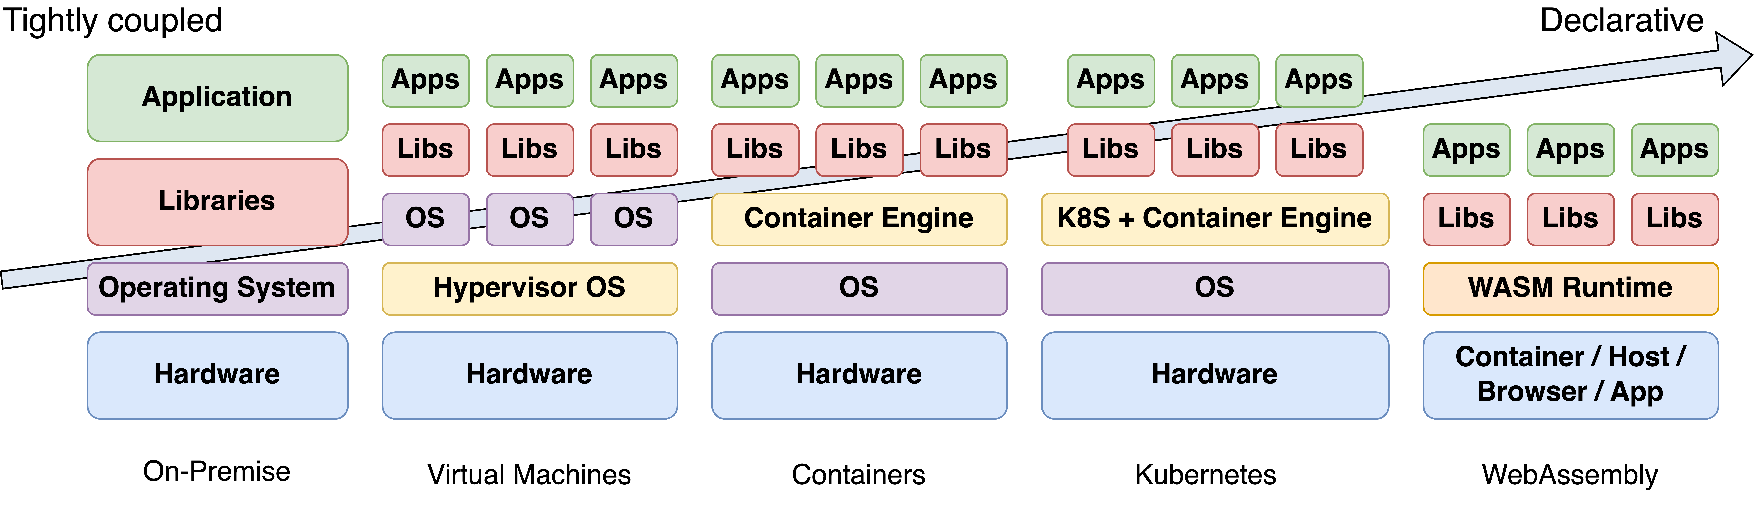
\includegraphics[width=\textwidth,height=\textheight,keepaspectratio]{images/introduction/Cloud_Transformation.pdf}
	\caption{Evolution of computation from on-premise to Wasm based on \cite{randall_2021_wasmcloud}}
	\label{fig:cloud-transformation}
\end{figure}

The figure \ref{fig:cloud-transformation} below depicts the evolution of \gls{cloud computing} from on premise model to the described WebAssembly serverless model.

Another promising browser technology is the usage of V8 \glspl{isolate}. According to Cloudflare, it achieves a startup time faster than a TLS handshake in under five seconds \cite{partovi_2020_eliminating}. The downside of isolates is that they can only execute JavaScript code. This thesis will compare both runtime technologies, but will focus on WebAssembly based runtime technologies.

\section{Research Objectives}
The goal of this research project is to evaluate various factors that affect performance and usability, among other things. Factors such as containerization, selection of WebAssembly runtime, and programming language will be emphasized. Considerations will be made regarding vendor lock-in, and potential strategies for avoiding it will be evaluated. Additionally, the paper will address interesting aspects such as sustainability in terms of resource conservation in the serverless domain. \\
\newline
Based on these requirements, the thesis aims to answer the following research question:
\begin{center}
\textit{"What are the effects of using WebAssembly technology in the serverless domain, particularly concerning the technologies employed (runtime environment, programming language), and how do they compare to existing solutions?"}
\end{center}


\section{Structure of the Thesis}

The remainder of this thesis is organized as follows:
\begin{itemize}
  \item Chapter 2 describes the current state of WebAssembly, including the current specification and any implemented proposals, as well as future proposals. It also covers the WebAssembly System Interface (WASI).
  \item Chapter 3
  \item Chapter 4
  \item Chapter 5
  \item Chapter 6
  \item Chapter 7
  \item Chapter 8
  \item Chapter 9
\end{itemize}

\chapter{WebAssembly (Wasm)}
\label{chap:wasm}
Since the dot-com era, JavaScript has remained the only client-side language for web browsers. As the web platform gained popularity and its standard APIs expanded, developers became increasingly interested in using faster programming languages on the web. To run these languages on the web, they had to be compiled into a common format, in this case, JavaScript. However, JavaScript, a high-level, dynamically typed, interpreted language, was not intended for this purpose, leading to performance issues.

In 2013, Mozilla engineers introduced a solution called asm.js, which focused on the parts of JavaScript that could be optimized ahead of time. This enabled C/C++ programs to be compiled into the asm.js target format and executed using a JavaScript runtime, achieving faster performance than equivalent JavaScript programs. However, benchmarks revealed that asm.js code ran about 1.5 times slower than the native code written in C++ \cite{zakai_2013_gap}.

As the need for improved web performance persisted, asm.js was replaced by WebAssembly (wasm), introduced in 2015.
“WebAssembly (abbreviated \Gls{WebAssembly}) is a safe, portable, low-level code format designed for efficient execution and compact representation. Its main goal is to enable high performance applications on the Web, but it does not make any Web-specific assumptions or provide Web-specific features, so it can be employed in other environments as well \cite[p.~1]{webassemblycommunitygroup_2023_webassembly}.”
The Wasm standard is developed by W3C Working Group and W3C Community Group. 

\section{Performance}


% \begin{itemize}
%   \item \textbf{Fast}: 
%   \item \textbf{Safe}:
%   \item \textbf{Well-defined}:
%   \item \textbf{Hardware-independent}:
%   \item \textbf{Language Agnosticism}:
%   \item \textbf{Platform-independent}:
% \end{itemize}

\section{Specification}
\label{sec:specification}

phases: \footnote{\url{https://github.com/WebAssembly/meetings/blob/main/process/phases.md}}

\section{Implemented proposals}
\label{sec:implemented-proposals}

\subsection{Multi-Value Return}
In modern programming languages that support tuples, like Kotlin, Rust or Python, developers can effortlessly bundle several values into a single structure for returning from a function. Simple tasks, such as switching a pair of values or sorting an array, become challenging since they must be performed within the linear memory block. Some arithmetic functions, including modular operations and carry bits, can also yield multiple values.

Apart from function return values, another limitation in the WebAssembly MVP is that instruction sequences, such as conditional blocks and loops, cannot consume or return more than one result. It would be equally intriguing to exchange values, perform arithmetic with overflow, or receive a multi-value tuple response in these scenarios as well. Furthermore, compilers are no longer required to jump through hoops when generating multiple stack values for core WebAssembly. This results in smaller generated bytecode and consequently, faster loading times.

\begin{lstlisting}[frame=lines, caption=Simple swap function that evaluates the multi return proposal, captionpos=b, language=JavaScript, showstringspaces=false]
(module
  (func $swap (import "" "swap") (param i32 i32) (result i32 i32))

  (func $mySwapfunc (export "mySwapfunc") (param i32 i32) (result i32 i32)
    (call $swap (local.get 0) (local.get 1))
  )
)
\end{lstlisting}

\subsection{Reference Types}

\subsection{Bulk Memory Operations}


\section{Future proposals}
\label{sec:future-proposals}

\section{Wasm bindgen}
\label{sec:wasm-bindgen}

\section{WebAssembly System Interface (WASI)}
\label{sec:wasi}
While WebAssembly is primarily designed for efficient operation on the web, as previously mentioned, it avoids making web-specific assumptions or integrating web-specific features. The core WebAssembly language remains independent of its surrounding environment and interacts with external elements exclusively through APIs. When operating on the web, it seamlessly utilizes existing web APIs provided by browsers. However, outside the browser environment, there is currently no standardized set of APIs for developing WebAssembly programs. This lack of standardization poses challenges in creating truly portable WebAssembly programs for non-web applications.

The WebAssembly System Interface (abbriveated as WASI) in short is a standard interface for WebAssembly modules to interact with their host environments, such as operating systems, without being tied to any specific host. This allows WebAssembly modules to be executed securely and portably across a wide range of environments. 

% State of WASI
According to Dan Gohman's proposed roadmap, the development of WASI is set to progress through Preview1, Preview2, and Preview3. Presently, the community is actively working on Preview2, ensuring that each milestone contributes to the ultimate goal of a stable and robust WASI 1.0 release. 

\begin{figure}[H]
	\centering
		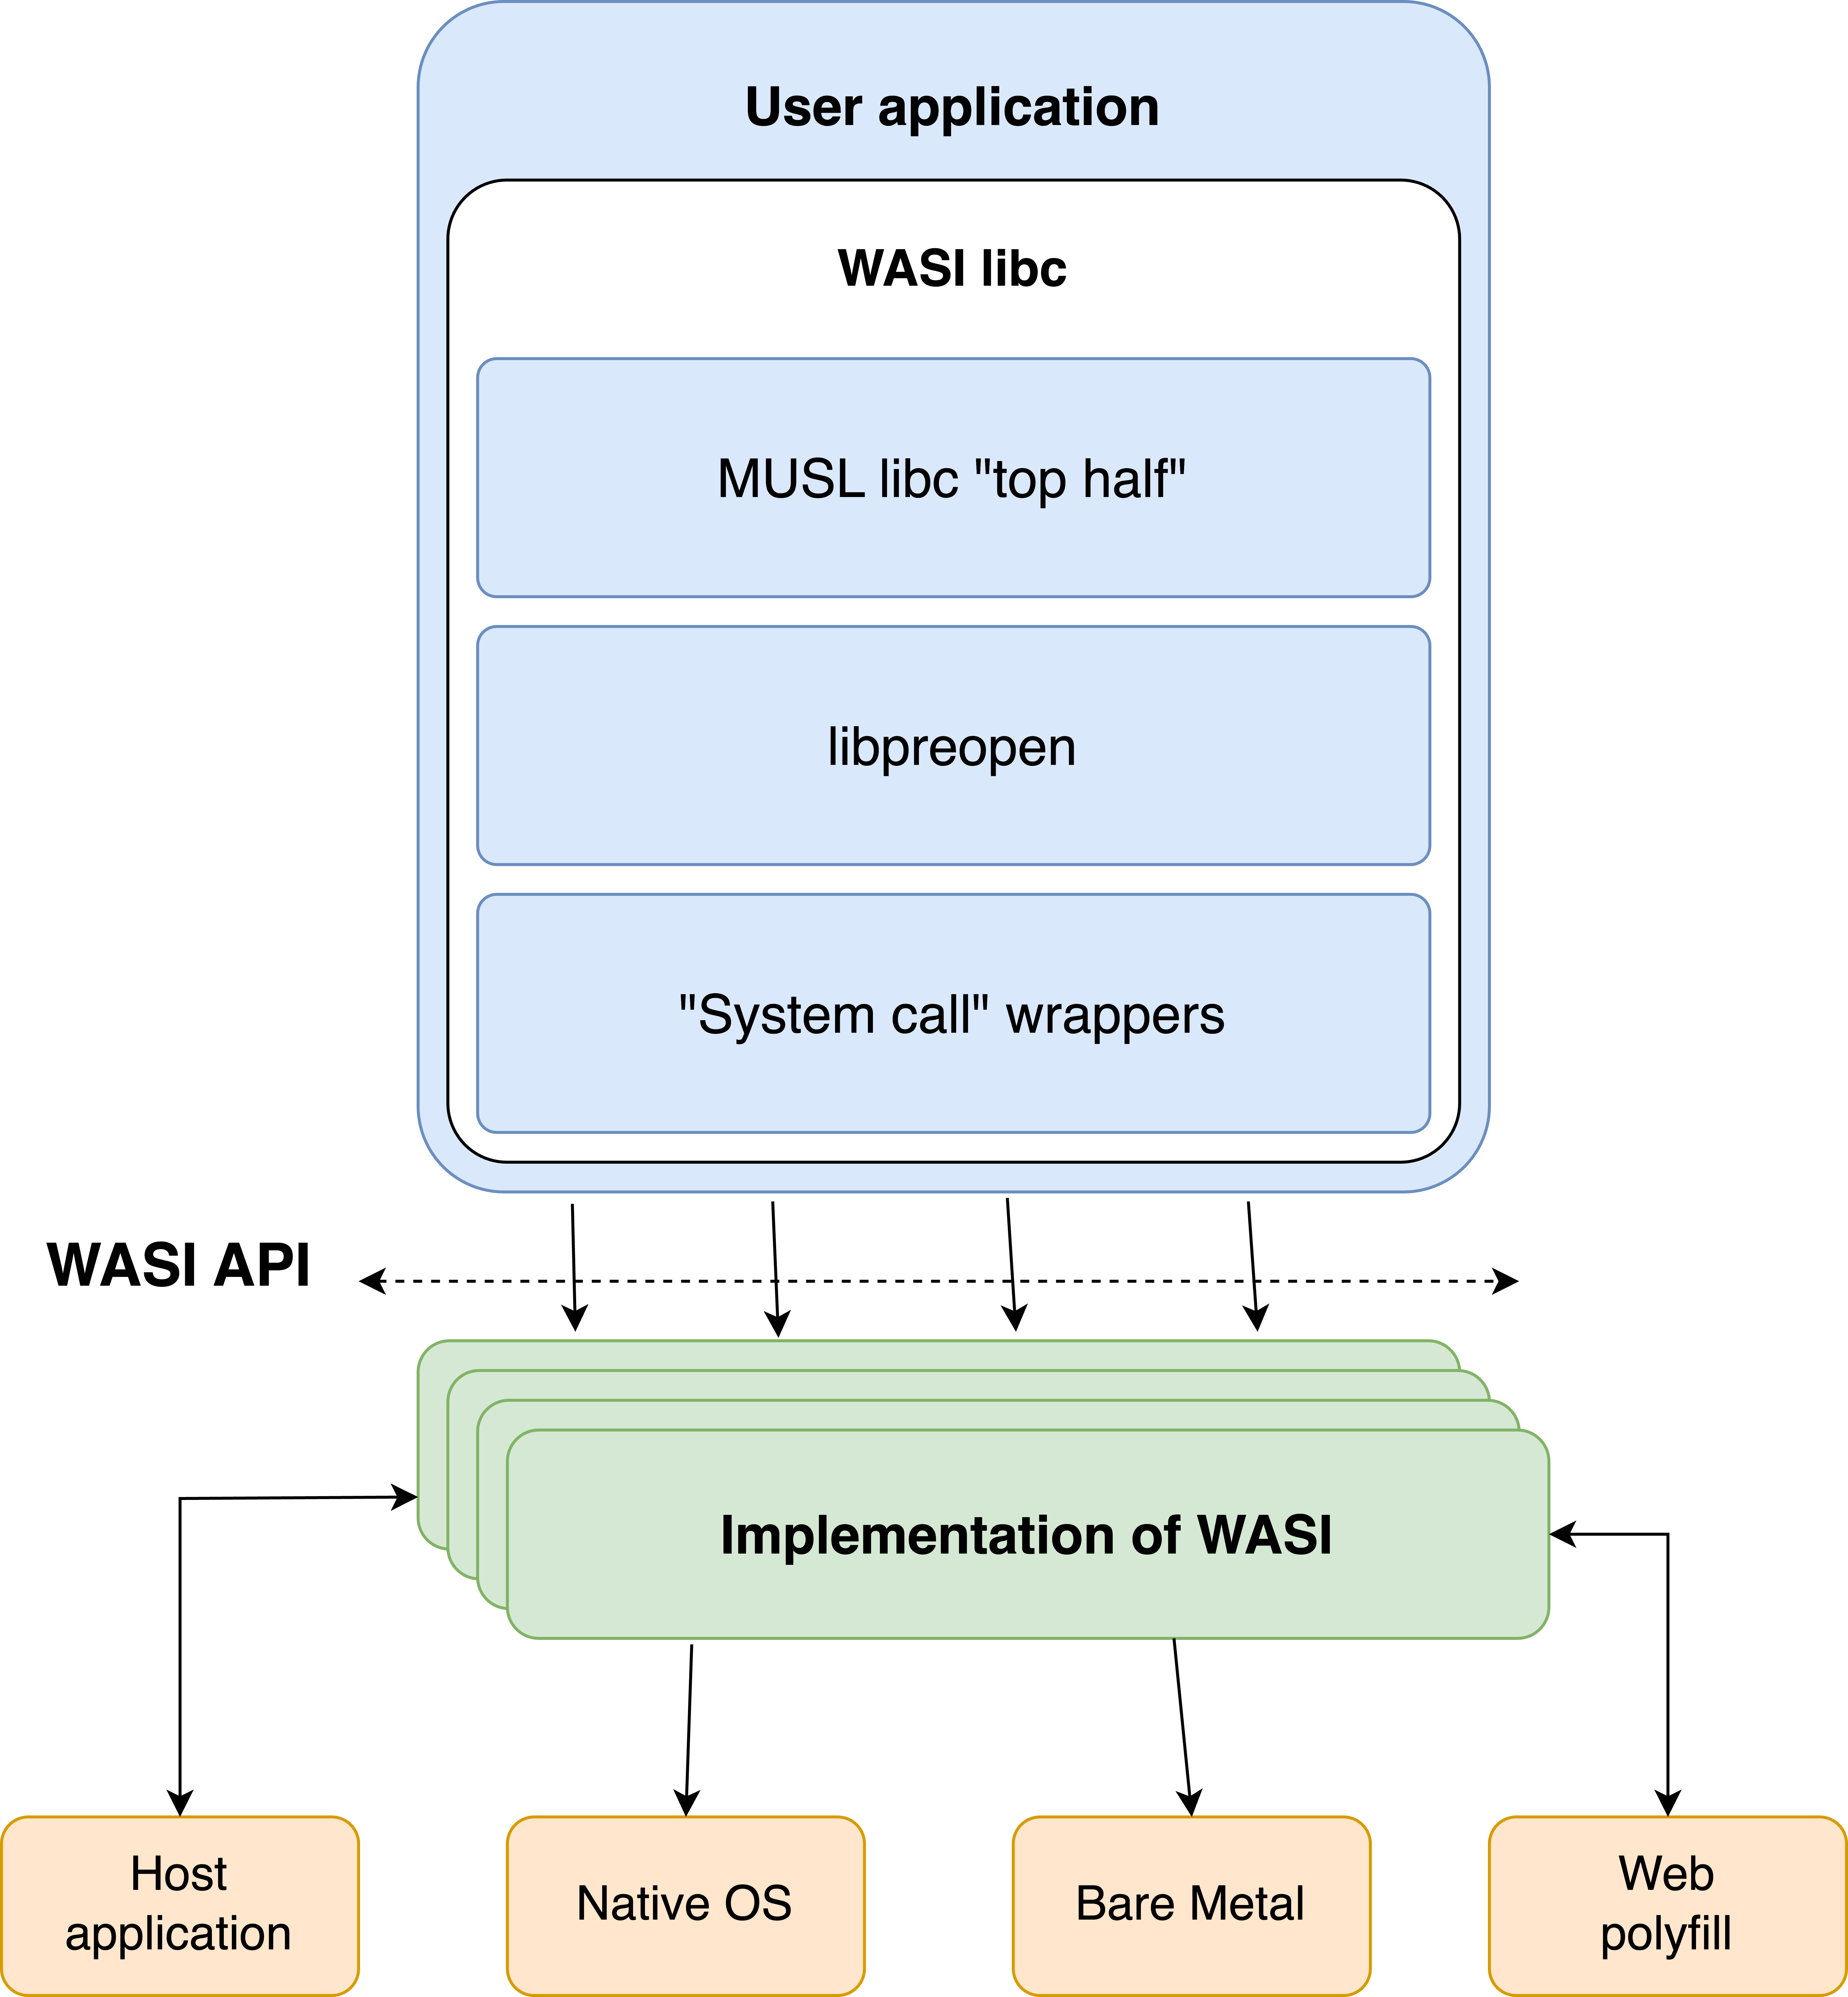
\includegraphics[width=130mm,scale=0.8]{images/wasm/WASI_Architecture.png}
	\caption{WASI Architecture}
	\label{fig:wasi-architecture}
\end{figure}

\subsection{WASI as Emscripten replacement?}
The first toolchain that enabled C, C++, or any other language with \gls{LLVM} support to be compiled into WebAssembly was Emscripten. Essentially, Emscripten can compile almost any portable C or C++ codebase into WebAssembly, encompassing high-performance games requiring graphics rendering, sound playback, and file loading and processing, as well as application frameworks like Qt. Emscripten has been utilized to convert numerous applications like Unreal Engine 4 and the Unity engine, into WebAssembly \cite{emscriptencommunity_2023_emscripten}. 

To achieve this, Emscripten implemented the \gls{POSIX} OS system interface on the web. As a result, developers are able to use the functions available in the C standard library (\gls{libc}). 
Emscripten accomplished this by creating its own implementation of libc, which was divided into two parts. One part was compiled into the WebAssembly module, while the other part was implemented in \gls{JS glue code}. The JS glue would subsequently communicate with the browser, which would in turn communicate with the Kernel and the OS.

\begin{figure}[H]
    \centering
        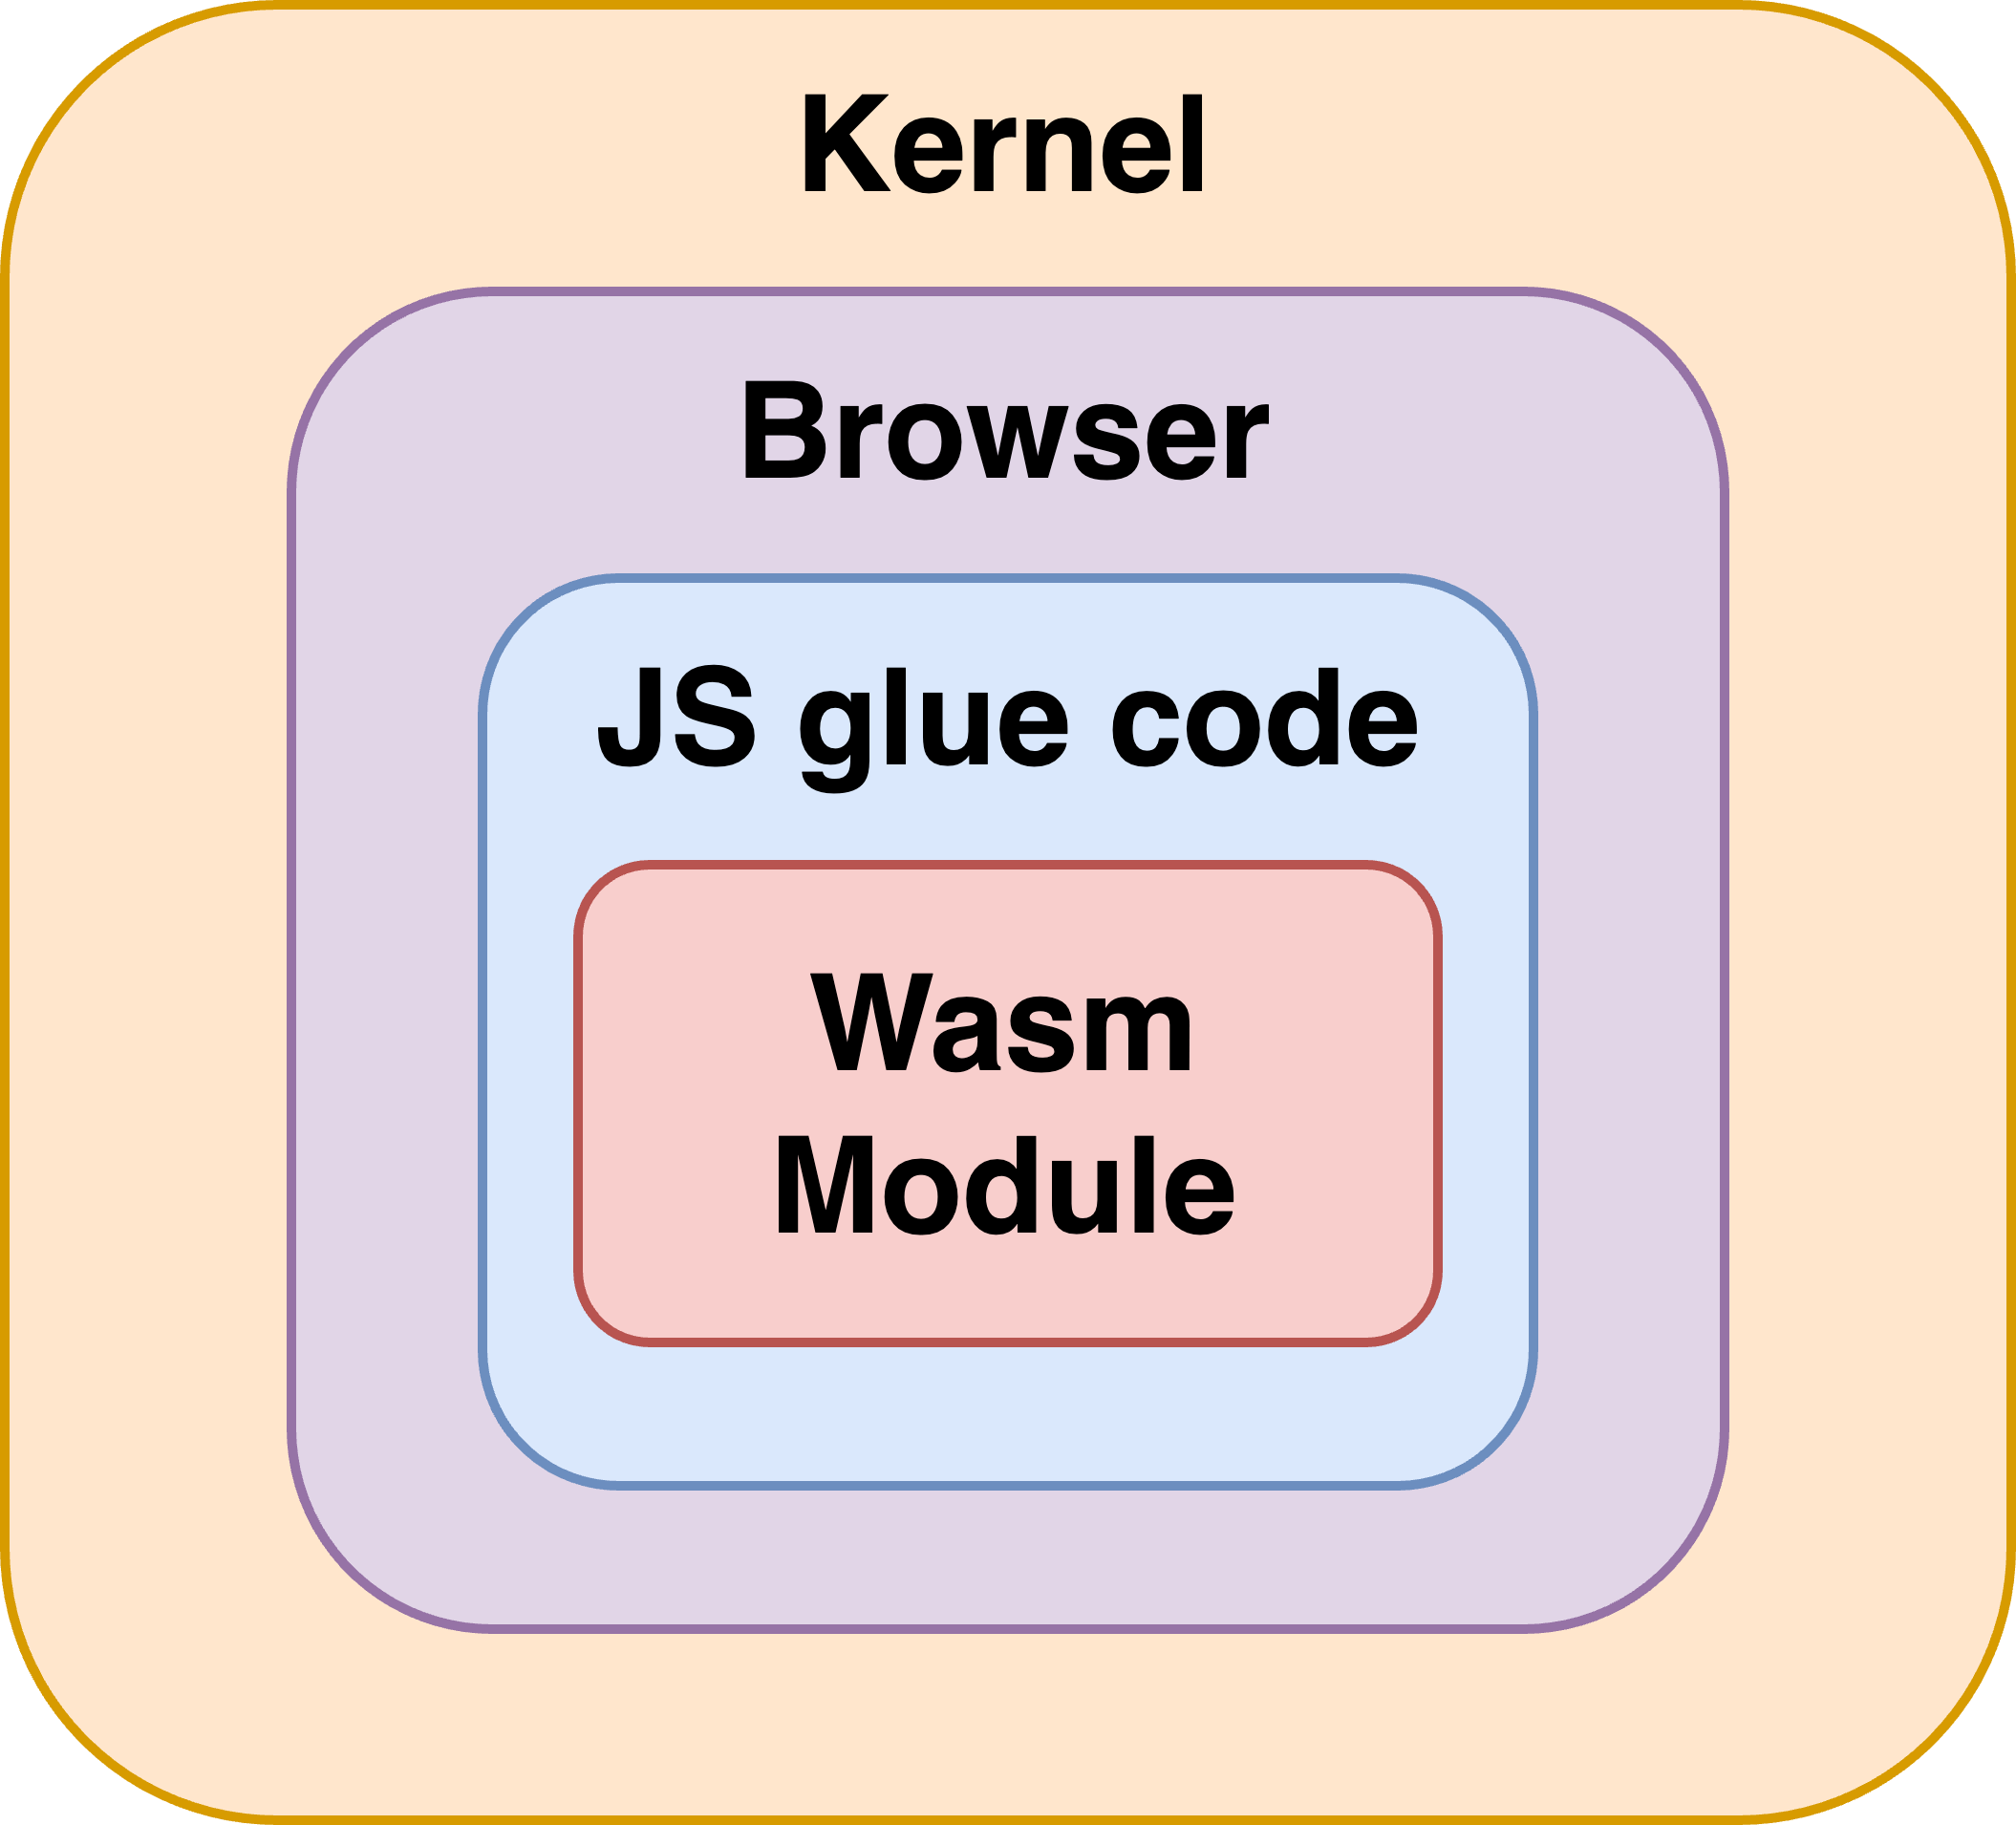
\includegraphics[width=0.6\linewidth]{images/wasm/Emscripten.png}
    \caption{Structure of Emscripten compiled Wasm module}
    \label{fig:emscripten}
\end{figure}

When users began to seek ways of running WebAssembly outside of a browser environment, the first approach was to enable the execution of Emscripten-compiled code on the corresponding environment.
To achieve this, the runtimes had to develop their own implementations of the functions in the JS glue code. However, this presented a challenge as the interface provided by the JS glue code was not intended to be a standard or public-facing interface. It was designed to serve a specific purpose, and creating a portable interface was not part of its intended design. The above figure \ref{fig:emscripten} shows the connection between the browser, the glue code and the Wasm module. 

Emscripten aims to improve the standard by using WASI APIs as extensively as possible in order to minimize unnecessary API differences. As previously stated, Emscripten code accesses Web APIs indirectly via JavaScript on the web. By making the JavaScript API resemble WASI, an unnecessary API difference can be eliminated, allowing the same binary to run on a server as well. In simpler terms, if a Wasm application wants to log information, it must call into JavaScript, following a process similar to this:

\verb|wasm => function musl_writev(...) { ... console.log(...) ... }|

"musl\_writev" represents an implementation of the Linux syscall interface utilized by "musl libc" to write data to a file descriptor, ultimately leading to a call to console.log with the appropriate data. The Wasm module imports and invokes "musl\_writev", thereby defining an ABI between the JavaScript and Wasm components. This ABI is arbitrary, by changing the existing ABI with one that aligns with WASI, the following can be achieved:

\verb|wasm => function __wasi_fd_write(...) { ... console.log(...) ... }|

% X 1. die API zu einem gewissen grad vereinheitlichen kann
% 2. es gibt dinge die emscripten machen kann aber wasi nicht macht
% 3. es macht vielleicht auch sinn eine api für web eine api für server und andere api's für plugins zu haben

%According to \cite{zakai_2019_outside} 

\subsection{WASI Portability}

\begin{figure}[H]
    \centering
        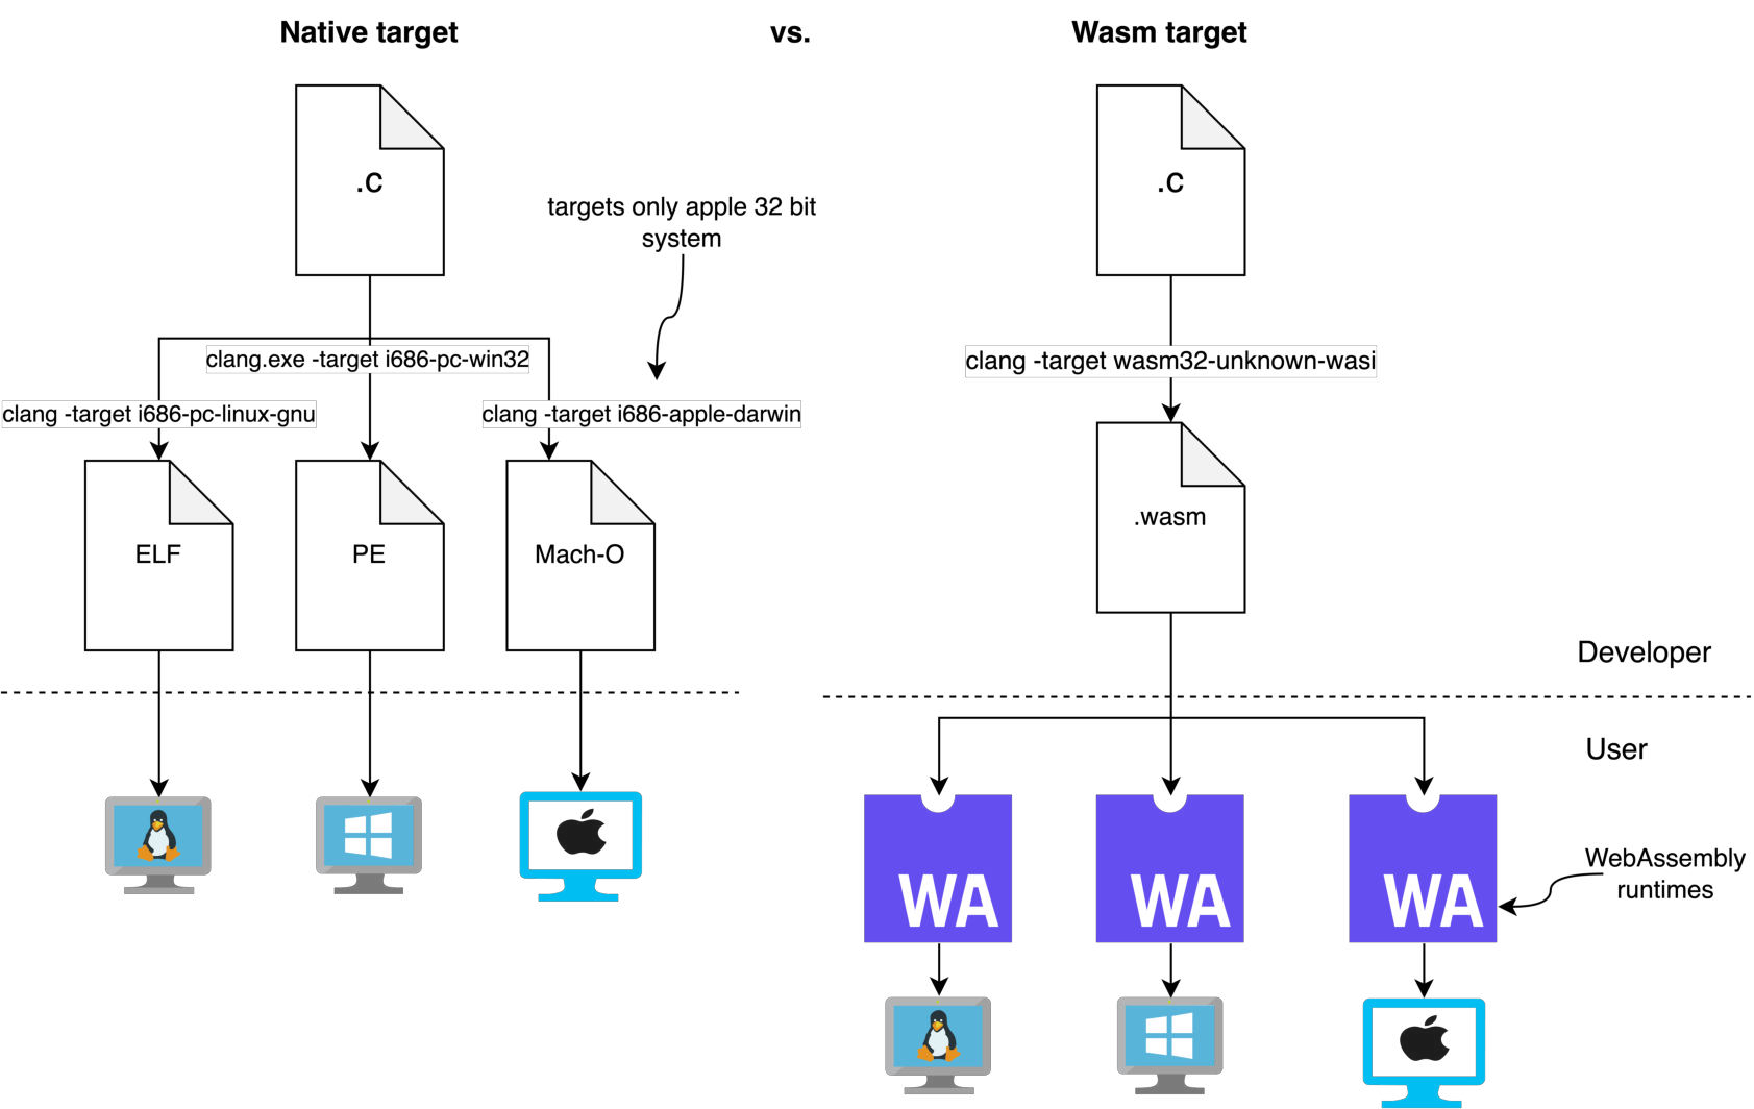
\includegraphics[width=1\linewidth]{images/wasm/WASI_PORTABILITY.pdf}
    \caption{WASI portability model redrawn from \cite{clark_2019_standardising}}
    \label{fig:wasi-portability}
\end{figure}


\subsection{WASI Security Model}
An essential aspect of any system is the security model implemented to ensure the integrity and confidentiality of data and resources. When a code segment requests the operating system (OS) to perform input or output operations, the OS must ascertain whether the action is secure and permissible.

Operating systems generally employ an access control mechanism based on ownership and group associations to manage security. For instance, consider a scenario where a program seeks permission from the OS to access a specific file. Each user possesses a unique set of files they are authorized to access. In Unix systems, for example, the ownership of a file can be assigned to three classes of users: user, group, and others.

Upon initiating the program, it operates on behalf of the respective user. Consequently, if the user has access to the file—either as the owner or as a member of a group with access rights—the program inherits the same privileges. This approach to security helps maintain a robust and reliable system that adheres to the principles of access control and resource protection.

This approach was effective in multi-user systems where administrators controlled software installation, and the primary threat was unauthorized user access. However, in modern single-user systems, the main risk comes from the code that the user runs, which often includes third-party code of unknown trustworthiness. This raises the risk of a supply chain attack, particularly when new maintainers take over open-source libraries, as their unrestricted access could enable them to write code that compromises system security by accessing files or sending them over the network \cite{clark_2019_standardising}.

 % explain supply chain attack

The security aspect of WASI is vital to the universal nature of WebAssembly. The WASI standard was built on a capabilities-based security model, which means the host has to explicitly permit capabilities such as file system access and establishing network sockets. As a result, a WASI module cannot run arbitrary code with direct access to memory.

% todo reference to a filesystem example wasmtime and wasmer



\chapter{Runtimes}
\label{chap:runtimes}


\section{Evaluation of features}
\label{sec:evaluation-of-features}

\subsection{JIT - Just In Time Compilation}
\label{sec:jit}

\subsection{Interpreter}
\label{sec:interpreter}

\subsection{WASM to native compilation}
\label{sec:wasm-to-native}

\subsection{AOT - Ahead Of Time Compilation}
\label{sec:aot}


 \subsection{Javascript snapshotting (Wizer)}
\label{sec:wizer}

\section{Comparison to V8 Isolates}
\label{sec:v8-comparison}
A V8 isolate is a separate instance of the V8 engine that has its own memory, garbage collector, and global object \cite{a2021_isolate}. An isolate can run scripts in a safe and isolated environment, without interfering with other isolates \cite{cloudflareinc_2023_how}. An isolate also has its own state, which means that objects from one isolate cannot be used in another isolate. When V8 is initialized, a default isolate is created and entered, but you can also create your own isolates using the V8 API \cite{a2021_isolate}.

\begin{figure}[htbp]
	\centering
		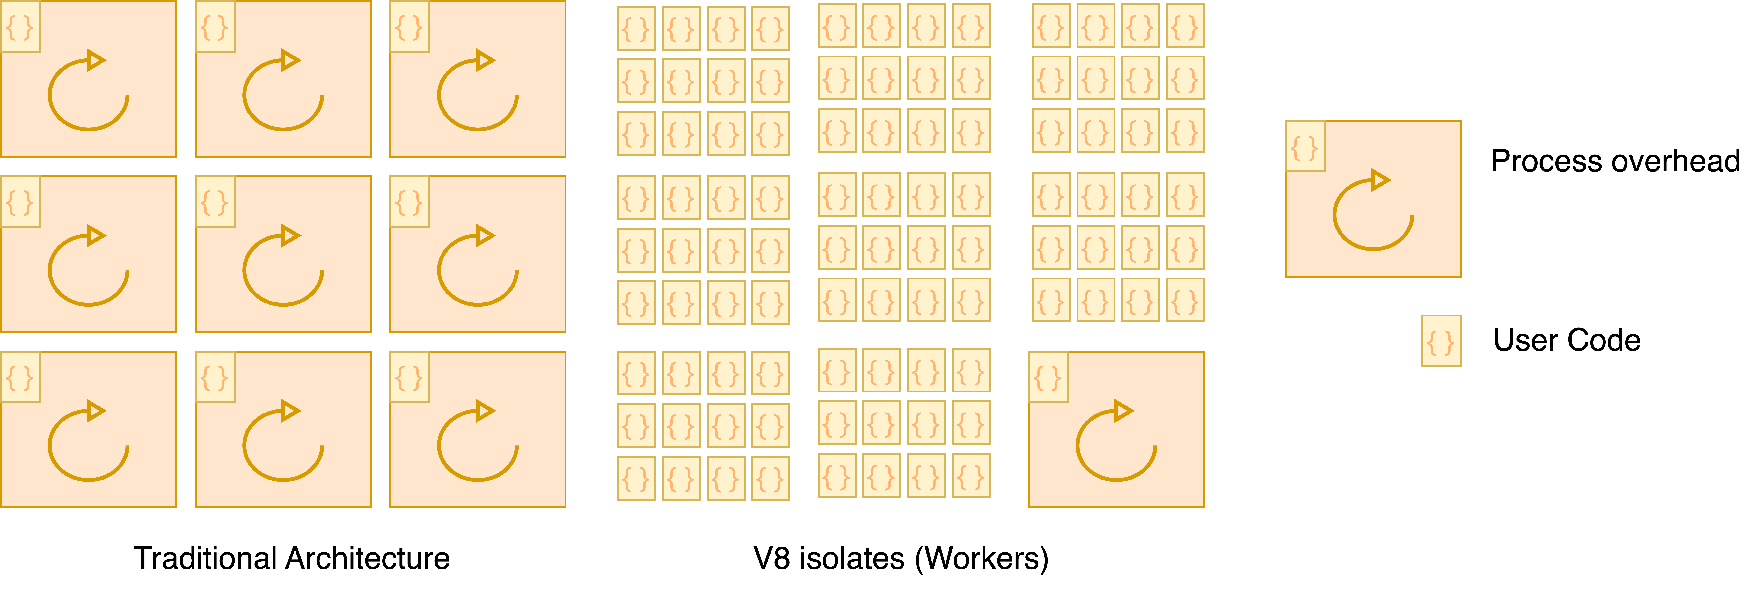
\includegraphics[width=\textwidth,height=\textheight,keepaspectratio]{images/runtimes/v8-isolates.pdf}
	\caption{containerized vs. \gls{V8} \glspl{isolate} figure redrawn from \cite{cloudflareinc_2023_how}}
	\label{fig:v8-isolates}
\end{figure}

\subsection{Advantages and disadvantages}
\label{sec:advantages-disadvantages}

\chapter{Simple POC WebAssembly Serverless Platform}
\label{chap:poc}
In this chapter, the proof of concept for a simple serverless platform using WebAssembly technology will be explored. The platform utilizes an HTTP server to direct HTTP requests to specific WebAssembly modules. The popular Rust web framework, "Actix-web," has been chosen for the HTTP server implementation due to its lightweight and fast nature. Furthermore, the proof of concept employs Wasmtime as the Wasm-WASI runtime. As mentioned in the previous chapter, Wasmtime offers excellent support for the WASI standard and integrates various programming languages such as C++, Rust, Go, JavaScript, and more.

As Figure \ref{fig:poc} illustrates, this proof of concept assumes the availability of a function registry service that stores the ahead-of-time compiled Wasm binaries. Additionally, a serverless platform needs to be distributed; therefore, API gateways and load balancers are necessary to serve requests across the network. However, this proof of concept primarily focuses on the WebAssembly aspect of the platform, leaving the API gateway and load balancers outside the scope of the discussion.

\begin{figure}[H]
	\centering
		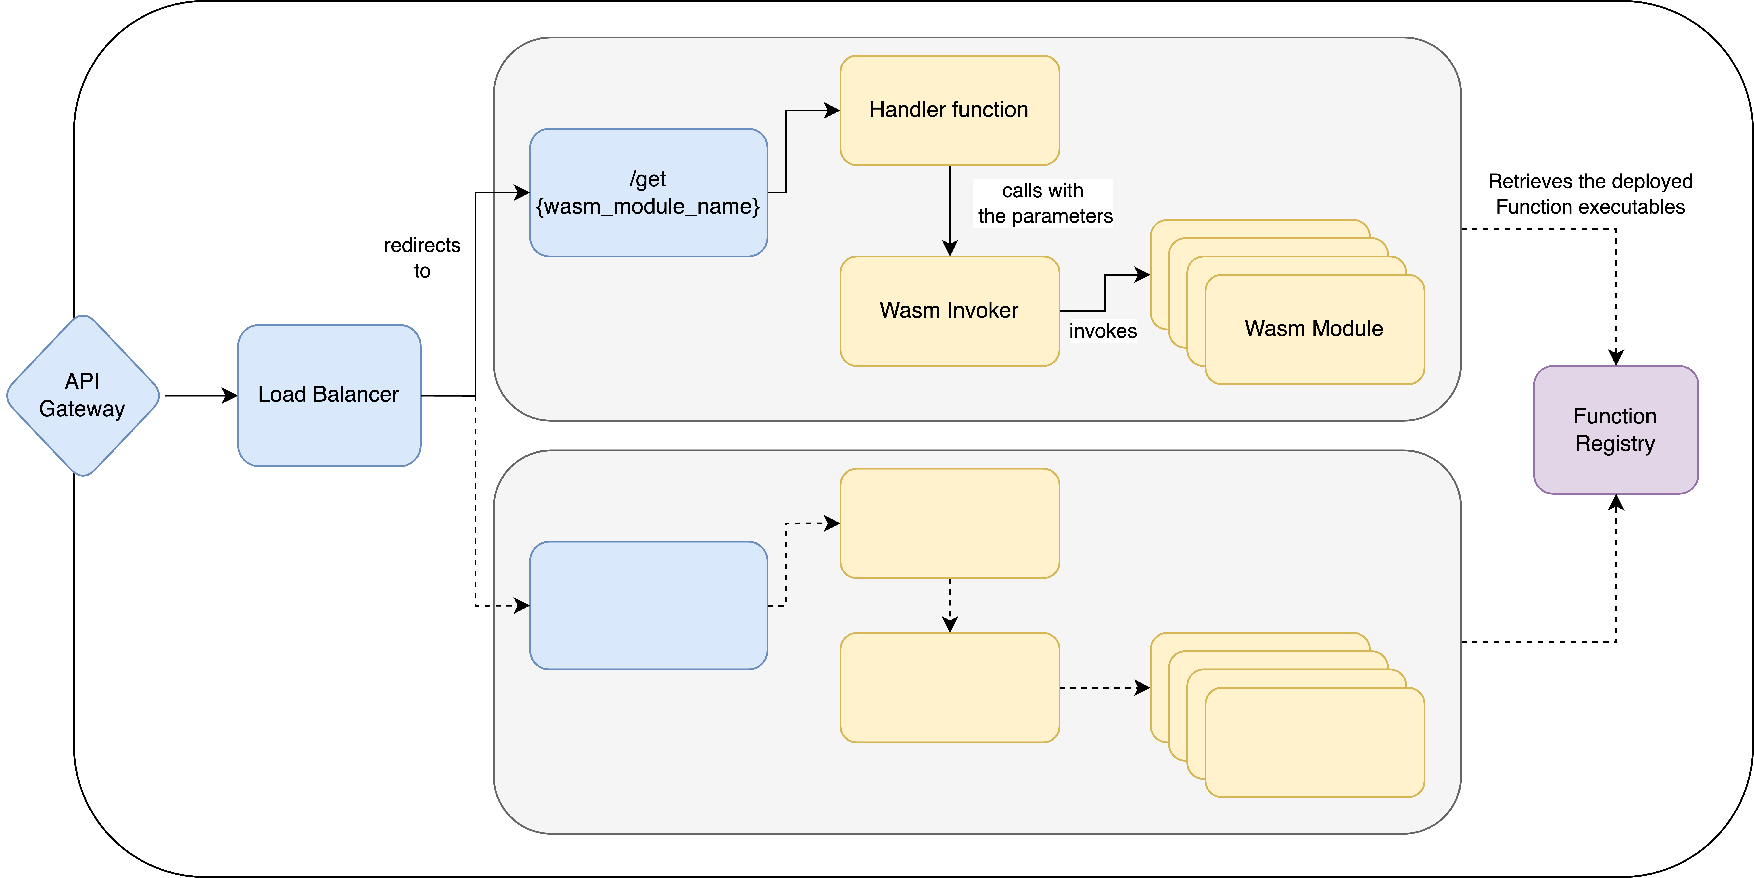
\includegraphics[width=1\linewidth]{images/poc/poc.pdf}
	\caption{Execution flow of the simple POC serverless platform}
	\label{fig:poc}
\end{figure}

%For this we need a WASI compliant Wasm modules, the fibonacci function from the previous chapter can be used here


\begin{lstlisting}[frame=lines, caption=actix http server with a handler function to invoce the wasm modules, captionpos=b, language=JavaScript, showstringspaces=false]
#[actix_web::main]
async fn main() -> io::Result<()> {
    HttpServer::new(|| App::new().service(handler))
        .bind("127.0.0.1:8080")?
        .run()
        .await
}

#[get("/{wasm_module_name}")]
async fn handler(
    wasm_module_name: Path<String>,
    query: Query<HashMap<String, String>>,
) -> impl Responder {
    let wasm_module = format!("{}.wasm", wasm_module_name);
    match invoke_wasm_module(wasm_module, query.into_inner()) {
        Ok(val) => HttpResponse::Ok().body(val),
        Err(e) => HttpResponse::InternalServerError().body(format!("Error: {}", e)),
    }
}

fn run_wasm_module(
    mut store: &mut Store<WasiCtx>,
    module: &Module,
    linker: &Linker<WasiCtx>,
) -> Result<()> {
    let instance = linker.instantiate(&mut store, module)?;
    let instance_main = instance.get_typed_func::<(), ()>(&mut store, "_start")?;
    Ok(instance_main.call(&mut store, ())?)
}
\end{lstlisting}


%Each stored Wasm module on the server is exposed by the handler function route, that takes the name of the Wasm module as a path parameter and loads the corresponding module.




\chapter{Benchmarks}
\label{chap:benchmarks}
\input{sections/5_benchmarks}

\chapter{Platform Limitations}
\label{chap:limitations}


The component model

\chapter{Vendor lock-in}
\label{chap:vendor-lock-in}
Cloud computing's vendor lock-in issue arises when customers become reliant (i.e., locked-in) on a specific cloud provider's technology implementation. This makes it challenging and costly to switch to another vendor due to legal constraints, technical incompatibilities, or significant expenses in the future. The issue of vendor lock-in in cloud computing has been identified as a major challenge because transferring applications and data to other providers is often an expensive and time-consuming process, making portability and interoperability essential considerations \cite{guest_2013_oracle}.

There are two primary factors contributing to the difficulty of achieving interoperability, portability, compliance, trust, and security in cloud computing. The first is the absence of universally adopted standards, APIs, or interfaces that can leverage the ever-changing range of cloud services. The second is the lack of standardized practices for deployment, maintenance, and configuration \cite{oparamartins_2014_critical}, which creates challenges for ensuring consistency and compatibility across cloud environments. 

\section{Key Motivations for shifting to a new Cloud Provider}
There are various reasons why a customer may contemplate changing their service provider:

\begin{enumerate}
    \item Inconsistent or unreliable service quality
    \item Escalating costs associated with function execution, prompting a search for a more cost-effective alternative.
    \item Runtime issues or limitations encountered with the current provider.
    \item The need to integrate a function with a new back-end service that is only offered by a different provider.
    \item Strategic or support considerations within the organization that may necessitate a switch to a different Cloud provider.
\end{enumerate}

\subsection{Service interoperability}


\subsection{Which parts need to be considered when migrating to a different provider?}
To evaluate the feasibility of switching \Gls{FaaS} providers, it is necessary to examine the modifications needed for the function codebase as well as the adjustments required for the execution configuration, deployment, and triggers.

\subsubsection{Differences in handler function}
Each cloud computing service provider has its own unique function signature that must be adhered to for the code to be executed on their respective cloud platforms. These signatures can vary slightly between different providers. The subsequent Javascript code examples illustrate how input can be read from the event and responses can be sent back for each cloud provider. These examples assume that the function is triggered through an HTTP POST request and with a JSON body conaining "myName" property. \\
The first example is an AWS Lambda Function, the body is within the event object, the function resolves the request by returning an object that contains a "statusCode" property along with a body.

\begin{lstlisting}[frame=lines, caption=Basic AWS Lambda Function, captionpos=b, language=JavaScript, showstringspaces=false]
export const handler = async(event, context) => {
    const input = JSON.parse(event.body);
    return {
        statusCode: 200,
        body: JSON.stringify({
            message: `Hello ${input.myName}`,
        })
    };
};
\end{lstlisting}
The next \gls{serverless} function is running on Google Cloud, the difference is not only in the function signature, but also the fact that the function imports the framework.

\begin{lstlisting}[frame=lines, caption=Basic Gen. 2 Google Cloud Functions, captionpos=b, language=JavaScript, showstringspaces=false]
const functions = require("@google-cloud/functions-framework");

functions.http("/", (req, res) => {
  res.status(200).send({
       message: `Hello ${req.body.myName}`
    });
});
\end{lstlisting}

TODO: short description

\begin{lstlisting}[frame=lines, caption=Basic Cloudflare Workers, captionpos=b, language=JavaScript, showstringspaces=false]
export default {
    async fetch(request, env, ctx) {
        const input = JSON.parse(await request.text());
        return new Response(JSON.stringify({
            message: `Hello, ${input.myName}`,
        }), {
            status: 200,
            headers: {
                "content-type": "application/json",
            },
        });
    },
};
\end{lstlisting}

TODO: short description

\begin{lstlisting}[frame=lines, caption=Basic Fastly Compute@Edge, captionpos=b, language=JavaScript, showstringspaces=false]
addEventListener("fetch", (event) => event.respondWith(handleRequest(event)));

async function handleRequest(event) {
  const request = event.request;
  const input = JSON.parse(await request.text());
  return new Response(JSON.stringify({
    message: `Hello, ${input.myName}`,
  }), { 
    status: 200,
    headers: {
      "content-type": "application/json",
    },
  });
}
\end{lstlisting}

\section{Design principles}
\subsection{Facade pattern}
The \gls{facade} pattern can be used as a mitigation strategy to avoid or reduce \gls{serverless} vendor lock-in. By creating a facade layer between the serverless function and the vendor-specific implementation, it is possible to decouple the function from the vendor's specific implementation details.
The facade layer provides a simplified interface that abstracts the underlying vendor implementation, allowing developers to write code that is agnostic to the specific \gls{serverless} vendor. If the vendor needs to be changed, the facade layer can be modified to adapt to the new vendor-specific implementation without affecting the business logic or the interface of the serverless function. This way, the codebase remains modular, and changing vendors becomes a relatively straightforward task.

\subsection{Adapter pattern}
SvelteKit is a modern web framework that effectively demonstrates the use of the Adapter pattern for deployment. Before deploying a SvelteKit application, it must be adapted to the specific deployment target by selecting an appropriate adapter in the configuration. This allows the application to be bundled with the platform-specific configuration \cite{sveltecommunity_2023_adapter}. 
The code snippet below illustrates the adapter configuration of a SvelteKit application, which enables the framework to be adapted to various cloud providers and allows the community to create new adapters. In this case, the deployment target is a Cloudflare Workers \gls{serverless} function.

\begin{lstlisting}[frame=lines, caption=svelte.config.js SvelteKit adapter configuration, captionpos=b, language=JavaScript, showstringspaces=false]
import adapter from '@sveltejs/adapter-cloudflare-workers';
 
/** @type {import('@sveltejs/kit').Config} */
const config = {
  kit: {
    adapter: adapter({
      // adapter options go here
    })
  }
};
 
export default config;
\end{lstlisting}

\section{The role of Wasm Portability}

\chapter{Related Work}
\label{chap:related-work}
\input{sections/8_related-work}

\chapter{Conclusion}
\label{chap:conclusion}
\input{sections/9_conclusion}

\chapter{Future work}
\label{chap:future-work}
Future work ...

%\clearpage

% --- Bibliography ------------------------------------------------------
\newpage
%IEEE Citation [1]
\bibliographystyle{IEEEtran}
\bibliography{master_thesis}
%for alphanumeric citation eg.: [ABC19]
%\bibliographystyle{alpha}
\addcontentsline{toc}{chapter}{Bibliography}
%\clearpage

% --- Glossary ----------------------------------------------------

%\newpage
\label{chap:glossary}
\printglossary
\addcontentsline{toc}{chapter}{Glossary}
%\clearpage


% --- List of Figures ----------------------------------------------------

\newpage
\listoffigures
\addcontentsline{toc}{chapter}{List of Figures}
%\clearpage


% --- List of Tables -----------------------------------------------------

\newpage
\listoftables
\addcontentsline{toc}{chapter}{List of Tables}
%\clearpage

% --- Appendix A -----------------------------------------------------

\newpage
\backmatter
\appendix
\begin{appendices}
\chapter{Appendix}
\begin{lstlisting}[frame=lines, caption=Simple Proof of Concept Wasm Serverless Platform using Actix and Wasmtime, captionpos=b, language=JavaScript, showstringspaces=false]
use actix_web::{
    get,
    web::{Path, Query},
    App, HttpResponse, HttpServer, Responder,
};
use anyhow::Result;
use std::{
    collections::HashMap,
    io,
    sync::{Arc, RwLock},
};
use wasi_common::{pipe::WritePipe, WasiCtx};
use wasmtime::*;
use wasmtime_wasi::WasiCtxBuilder;

#[actix_web::main]
async fn main() -> io::Result<()> {
    HttpServer::new(|| App::new().service(handler))
        .bind("127.0.0.1:8080")?
        .run()
        .await
}

#[get("/{wasm_module_name}")]
async fn handler(
    wasm_module_name: Path<String>,
    query: Query<HashMap<String, String>>,
) -> impl Responder {
    let wasm_module = format!("{}.wasm", wasm_module_name);
    match invoke_wasm_module(wasm_module, query.into_inner()) {
        Ok(val) => HttpResponse::Ok().body(val),
        Err(e) => HttpResponse::InternalServerError().body(format!("Error: {}", e)),
    }
}

fn run_wasm_module(
    mut store: &mut Store<WasiCtx>,
    module: &Module,
    linker: &Linker<WasiCtx>,
) -> Result<()> {
    let instance = linker.instantiate(&mut store, module)?;
    let instance_main = instance.get_typed_func::<(), ()>(&mut store, "_start")?;
    Ok(instance_main.call(&mut store, ())?)
}

fn invoke_wasm_module(wasm_module_name: String, params: HashMap<String, String>) -> Result<String> {
    // create a wasmtime engine
    let engine = Engine::default();

    let mut linker = Linker::new(&engine);
    wasmtime_wasi::add_to_linker(&mut linker, |s| s)?;

    // create a buffer to store the response
    let stdout_buf: Vec<u8> = vec![];
    let stdout_mutex = Arc::new(RwLock::new(stdout_buf));
    let stdout = WritePipe::from_shared(stdout_mutex.clone());

    // convert params hashmap to an array
    let envs: Vec<(String, String)> = params
        .iter()
        .map(|(key, value)| (key.clone(), value.clone()))
        .collect();

    let wasi = WasiCtxBuilder::new()
        .stdout(Box::new(stdout))
        .envs(&envs)?
        .build();
    let mut store = Store::new(&engine, wasi);

    let module = Module::from_file(&engine, &wasm_module_name)?;
    linker.module(&mut store, &wasm_module_name, &module)?;

    run_wasm_module(&mut store, &module, &linker).unwrap();

    // read the response into a string
    let mut buffer: Vec<u8> = Vec::new();
    stdout_mutex
        .read()
        .unwrap()
        .iter()
        .for_each(|i| buffer.push(*i));
    let s = String::from_utf8(buffer)?;
    Ok(s)
}
\end{lstlisting}


\clearpage
\end{appendices}

\end{document}
